\documentclass[11pt]{article}
\usepackage[scaled=0.92]{helvet}
\usepackage{geometry}
\geometry{letterpaper,tmargin=1in,bmargin=1in,lmargin=1in,rmargin=1in}
\usepackage[parfill]{parskip} % Activate to begin paragraphs with an empty line rather than an indent %\usepackage{graphicx}
\usepackage{amsmath,amssymb, mathrsfs, dsfont, stackrel}
\usepackage{tabularx}
\usepackage[font=footnotesize,labelfont=bf]{caption}
\usepackage{graphicx}
\usepackage{xcolor}
%\usepackage[linkbordercolor ={1 1 1} ]{hyperref}
%\usepackage[sf]{titlesec}
\usepackage{natbib}
\usepackage{../../Tianpei_Report}
%\usepackage{appendix}
%\usepackage{algorithm}
%\usepackage{algorithmic}

%\renewcommand{\algorithmicrequire}{\textbf{Input:}}
%\renewcommand{\algorithmicensure}{\textbf{Output:}}



\begin{document}
\title{Lecture 6: Monte Carlo Optimization}
\author{ Tianpei Xie}
\date{Sep. 28th., 2022 }
\maketitle
\tableofcontents
\newpage
\allowdisplaybreaks
\section{Introduction}
\begin{itemize}
\item Similar to the problem of integration, differences between the numerical approach and the simulation approach to the problem
\begin{align}
\max_{\mb{x}\in \cX} h(\mb{x}) \label{eqn: stochastic_opt}
\end{align} lie in the treatment of the function $h$. 
\begin{itemize}
\item In approaching an optimization problem using deterministic numerical methods, the \emph{\textbf{analytical properties}} of the target function (\emph{convexity}, \emph{boundedness}, \emph{smoothness}) are often paramount.
\item For the simulation approach, we are more concerned with $h$ from a \emph{\textbf{probabilistic}} (rather than analytical) point of view. 
\end{itemize}

\item We want to distinguish between two approaches to \underline{\emph{\textbf{Monte Carlo optimization}}} \citep{robert1999monte}.
\begin{itemize}
\item  The first is an \underline{\emph{\textbf{exploratory approach}}}, in which the goal is to optimize the function $h$ by \emph{describing its entire range}. The \emph{actual properties} of the function play a \emph{lesser role} here, with the Monte Carlo aspect more closely tied to the \emph{\textbf{exploration of the entire space}} $\cX$, even though, for instance, the slope of $h$ can be used to speed up the exploration.

\item The second approach is based on a \underline{\emph{\textbf{probabilistic approximation}}} of the \emph{objective function} $h$ and is somewhat of a \emph{preliminary step} to the actual optimization. Here, the Monte Carlo aspect \emph{\textbf{exploits the probabilistic properties of the function}} $h$ to come up with an acceptable approximation and is less concerned with exploring $\cX$. For instance, \emph{Missing data methods}, such as the \emph{EM algorithm}, are closely related to tied to this idea.
\end{itemize}
\end{itemize}

\section{Stochastic Explorations}
\begin{itemize}
\item There are a number of cases where the exploration method is particularly well suited. For instance, when $\cX$ is bounded, we can use grid search, there the function $h$ is approximated by  $\mb{h}= [h(x_i)]_{i}$. Distributions other than the uniform, which can possibly be related to $h$, may then do better. In particular, in setups where the likelihood function is extremely costly to compute, the number of evaluations of the function $h$ is best kept to a minimum.

\item The second direction is to relates $h$ to a probability distribution. For instance, $h >0$ and $\int_{\cX} h(\mb{x}) d\mb{x} < \infty$, the resolution of \eqref{eqn: stochastic_opt} amounts to finding the \emph{\textbf{modes}} of the density $h$. More generally, if these conditions are not satisfied, then we may be able to transform the function $h(\mb{x})$ into another function $H(\mb{x})$ that satisfies the condition of positivity with finite integral. For instance $H(\mb{x}) :\propto \exp\paren{h(\mb{x})/T}$ or $H(\mb{x}) :\propto \sigma\paren{h(\mb{x})/T}$ where $\sigma(x) = 1/(1 + \exp(-x))$. We can choose $T$ to accelerate convergence or to avoid local maxima (\emph{Simulated Annealing}). 
\end{itemize}
\subsection{Gradient Methods}
\begin{itemize}
\item The gradient method is a \emph{deterministic} numerical approach to the problem \eqref{eqn: stochastic_opt}. It produces a sequence $(\mb{x}_{t})$ that converges to the exact solution of \eqref{eqn: stochastic_opt}, $\mb{x}^{*}$, when the domain $\cX \subseteq \bR^d$ and the function $(-h)$ are both \emph{convex}. The sequence $(\mb{x}_{t})$ is constructed in a \emph{\textbf{recursive}} manner through
\begin{align*}
\mb{x}_{t+1} &= \mb{x}_{t} + \alpha_{t}\grad{}{h(\mb{x}_t)}, \quad \alpha_t > 0.
\end{align*}

\item In more general setups (that is, when the function or the space is less regular), equation above can be modified by stochastic perturbations to again achieve convergence. One of these stochastic modifications is to choose a second sequence $(\beta_t)$ to define the chain  $(\mb{x}_{t})$ by
\begin{align}
\mb{x}_{t+1} &= \mb{x}_{t} + \frac{\alpha_{t}}{2\beta_{t}}\Delta\,h(\mb{x}_t, \beta_{t}\mb{\xi}_{t})\mb{\xi}_{t}, \quad \alpha_t > 0. \label{eqn: sgd}\\
\text{where }\Delta\,h(\mb{x}_t, \beta_{t}\mb{\xi}_{t}) &= \paren{h(\mb{x}_t + \beta_{t}\mb{\xi}_{t}) - h(\mb{x}_t - \beta_{t}\mb{\xi}_{t})} \approx 2\,\beta_{t}\norm{\mb{\xi}_{t}}{2}\grad{}{h(\mb{x}_t)}, \nonumber
\end{align} and the variables $\mb{\xi}_{t}$ are uniformly distributed on the unit sphere $\norm{\mb{\xi}_{t}}{2} = 1$.

In contrast to the deterministic approach, this method does not necessarily proceed along the \emph{steepest slope} in $(\mb{x}_{t})$, but this property is sometimes a \emph{plus} in the sense that it may \emph{avoid being trapped in \textbf{local maxima}} or in \emph{\textbf{saddlepoints}} of $h$.

\item Consider the objective function is the sample average of log-likelihood function 
$h(\mb{\theta}): = \sum_{i=1}^{N}\ell(\mb{\theta}; \mb{x}_i)$. The \emph{\textbf{stochastic gradient ascent}} is of form
\begin{align}
\mb{\theta}_{t+1} &= \mb{\theta}_{t} + \alpha_{t}\grad{\mb{\theta}}{\ell(\mb{\theta}_{t}; \mb{\xi}_t)}, \quad \alpha_t > 0.
\label{eqn: sgd_2}
\end{align} where $\mb{\xi}_{t} \sim \set{\mb{x}_1, \ldots, \mb{x}_{n}}$ is a random sample from data.
\end{itemize}

\subsection{Simulated Annealing}
\begin{itemize}
\item The \emph{\textbf{fundamental idea}} of \emph{\textbf{simulated annealing methods}} is that a change of scale, called \emph{\textbf{temperature}}, allows for faster moves on the surface of the function $h$ to maximize, whose negative is called \emph{\textbf{energy}}. Therefore, rescaling partially avoids the trapping attraction of local maxima.

\item Given a temperature parameter $T > 0$, $(\mb{X}_{t}^{(k)})$ is generated from the distribution
\begin{align}
\pi_{k}(\mb{x}) &\propto \exp\paren{\frac{h(\mb{x})}{T_{k}}}
\end{align} As $T_{k}$ decreases toward $0$, the values simulated from this distribution become concentrated in a narrower and narrower neighborhood of the \emph{local maxima} of $h$

\item In Simulated Annealing, we run a fixed number of $N_k$ iterations of MCMC (\emph{Metropolis-Hastings} or \emph{Gibbs sampling}) so that $(\mb{X}_t^{(k)})$ follows the stationary distribution $\pi_k(\mb{x}) \propto \exp(h(\mb{x})/T_{k})$. Then we decrease temperature $T_{k}$ to $T_{k+1}$ and restart the MCMC with last update $\mb{X}_{k}$. As $T_{k}\rightarrow 0$, the target distribution is approaching to an indicator on its mode, thus the simulated samples would be close to the optimal solution.


\item The \underline{\emph{\textbf{Simulated Annealing algorithm}}} can be implemented as 
\begin{enumerate}
\item Simulate $\mb{\xi}$ from an \emph{instrumental distribution} with density $g(\norm{\mb{\xi} - \mb{X}_{t}}{})$;
\item Accept $\mb{X}_{t+1} = \mb{\xi}$ with probability
\begin{align*}
\alpha(\mb{X}_t, \mb{\xi})&= \min\set{1, \exp\paren{\frac{\Delta h_{t}}{T_{t}}}}
\end{align*} where $\Delta h_t := h(\mb{\xi}) - h(\mb{X}_t)$;
\item Otherwise, accept $\mb{X}_{t+1} = \mb{X}_t$.
\item Update $T_{t}$ to $T_{t+1}$.
\end{enumerate}

\item  Since there is non-zero probability of accepting a new proposal even if it is not local maximal, it allows the algorithm to \emph{escape the attraction} of $\mb{x}_t$ if $\mb{x}_t$ is a local maximum of $h$. The temperature $T_{k}$ controls the probability of acceptance of non-optimal proposal.

\item An important feature of the simulated annealing algorithm is that there exist convergence results in the case of \textbf{finite spaces}. \citep{robert1999monte}

\item It can be shown that the global optimum of $h(\mb{x})$ can be reached by Simulated Annealing algorithm with probability $1$ if the temperature variable $T_k$ \textbf{decreases} \emph{\textbf{sufficiently slowly}}, i.e., at the order of $\cO(\log(L_k)-1)$, where $L_k = N_1 +\ldots + N_k$, $N_k$ is the number of iterations of MCMC at time $t$. In practice, however, no one can afford to have such a slow annealing schedule. Most frequently, people use a linear or even exponential temperature decreasing schedule, which can no longer guarantee that the global optimum will be reached \citep{liu2001monte}. 
\end{itemize}

\subsection{Simulated Tempering}
\begin{itemize}
\item \emph{\textbf{Simulated Tempering (ST)}} is proposed to let a MCMC scheme move more freely in the state space \citep{liu2001monte}.

\item Define a new target distribution, $\pi(\mb{x}, i) \propto c_{i}\exp\set{-h(\mb{x})/T_{i}}$ on the augmented space $(\mb{x}, i) \in \cX \times I$. Here, the $c_i$ are constants that can be controlled by the user and they should be tuned so that each tempered distribution in the system should have a roughly equal chance to be visited. Ideally, the $c_i$ should be proportional to the reciprocal of the $i$-th partition function, $Z_i = \int \exp\set{-h(\mb{x})/T_i}$.

\item The \underline{\emph{\textbf{Simulated Tempering (ST)}}} is described as 
\begin{enumerate}
\item With the current state $(\mb{X}_{t},\, i_{t}) = (\mb{x}, \,i)$, we draw $u\sim \cU[0,1]$.
\item (\emph{\textbf{Update sample}}) If $u \le \alpha_0$, we let $i_{t+l} = i$ and let $\mb{X}_{t+1}$ be drawn from a \emph{\textbf{MCMC transition}} $K_i(\mb{x}, \mb{x}_{t+1})$ that leaves $\pi_i\propto \exp(h(\mb{x})/T_{i})$ invariant.

\item (\emph{\textbf{Update temperature}}) If $u > \alpha_0$, we let $\mb{X}_{t+l} = \mb{x}$ and propose a \emph{\textbf{level transition}}, $i \rightarrow i'$, from a transition function $\alpha(i, i')$ (usually a nearest-neighbor simple random walk with reflecting boundary), and let $i_{t+1} = i'$ with probability
\begin{align*}
\min\set{1, \frac{c_{i'}\,\pi_{i'}(\mb{x})\,\alpha(i', i) }{ c_{i}\,\pi_i(\mb{x})\,\alpha(i, i')}};
\end{align*} otherwise accept $i_{t+1} = i$.
\end{enumerate} 
\end{itemize}

\section{Stochastic Approximations}
\subsection{The EM Algorithm}
\begin{itemize}
\item Missing data models are best thought of as models where the likelihood
can be expressed as
\begin{align}
g( \mb{y} | \mb{\theta} ) &= \int_{\cX} p(\mb{x}, \mb{y} | \mb{\theta}) d\mb{x} \label{en: missing_data}
\end{align} We refer to representation \eqref{en: missing_data} as \emph{\textbf{demarginalization}}.

\item The \emph{incomplete likelihood function} $\ell(\mb{\theta}|\mb{x})$ to be optimized can be expressed
as the expectation
\begin{align*}
\ell(\mb{\theta}|\mb{y}) &= \E{}{\ell_{c}(\mb{\theta}|\mb{y}, \mb{X})} = \int_{\cX}\ell_{c}(\mb{\theta}|\mb{x}, \mb{y})d\mb{x}
\end{align*} We refer to the function $\ell_{c}(\mb{\theta}|\mb{x}, \mb{y}) = p(\mb{x}, \mb{y} | \mb{\theta})$ as the \emph{complete-data likelihood}, which corresponds to the observation of the complete data $(\mb{x}, \mb{y})$. 

\item The \emph{\textbf{EM (Expectation-Maximization) algorithm}} was originally introduced by Dempster et al. (1977) to overcome the difficulties in maximizing likelihoods by taking advantage of the representation \eqref{en: missing_data} and solving a sequence of easier maximization problems whose limit is the answer to the original problem. 

\item In particular, we can obtain lower bound of incomplete log-likelihood
\begin{align*}
\log\ell(\mb{\theta}|\mb{y})  = \log \int_{\cX}p(\mb{x}, \mb{y} | \mb{\theta})d\mb{x} 
&= \log \int_{\cX} q(\mb{x}|\mb{y},\mb{\theta}) \frac{p(\mb{x}, \mb{y} | \mb{\theta})}{q(\mb{x}|\mb{y},\mb{\theta})}  d\mb{x} \\
&\ge \int_{\cX}q(\mb{x}|\mb{y},\mb{\theta})\log\frac{p(\mb{x}, \mb{y} | \mb{\theta})}{q(\mb{x}|\mb{y},\mb{\theta})}  d\mb{x}  \\
&= \E{q}{\ell_{c}(\mb{\theta}|\mb{x}, \mb{y})} - \E{q}{q(\mb{x}|\mb{y},\mb{\theta})}
\end{align*} Let $q(\mb{x}|\mb{y},\mb{\theta}):= \frac{p(\mb{x}, \mb{y} | \mb{\theta})}{g(\mb{y}| \mb{\theta})}$ be the condition distribution of latent variable given observed data. Common EM notation is to denote the expected log-likelihood by
\begin{align*}
Q(\mb{\theta}|\mb{\theta}_{0}, \mb{y}) &:= \E{\mb{\theta}_{0}}{\ell_{c}(\mb{\theta}|\mb{x}, \mb{y})} 
\end{align*} where $q(\mb{x}|\mb{y},\mb{\theta}_0)$ is the variational distribution.

Thus the EM algorithm contains two steps:
\begin{enumerate}
\item (E-Step): Compute $Q(\mb{\theta}|\mb{\theta}_{t}, \mb{y}) = \E{\mb{\theta}_{t}}{\ell_{c}(\mb{\theta}|\mb{x}, \mb{y})} $ with respect to $q(\mb{x}|\mb{y},\mb{\theta}_t)$
\item (M-Step): Optimize $q$ via $\mb{\theta}_{t+1} = \arg\max_{\mb{\theta}}Q(\mb{\theta}|\mb{\theta}_{t}, \mb{y})$
\end{enumerate}

\item It can be shown that EM algorithm increase the incomplete log-likelihood at each iteration:
\begin{align*}
\log\ell(\mb{\theta}_{t}|\mb{y}) \ge \log\ell(\mb{\theta}_{t-1}|\mb{y})
\end{align*}
\end{itemize}
\begin{figure}
\begin{minipage}[t]{1\linewidth}
  \centering
  \centerline{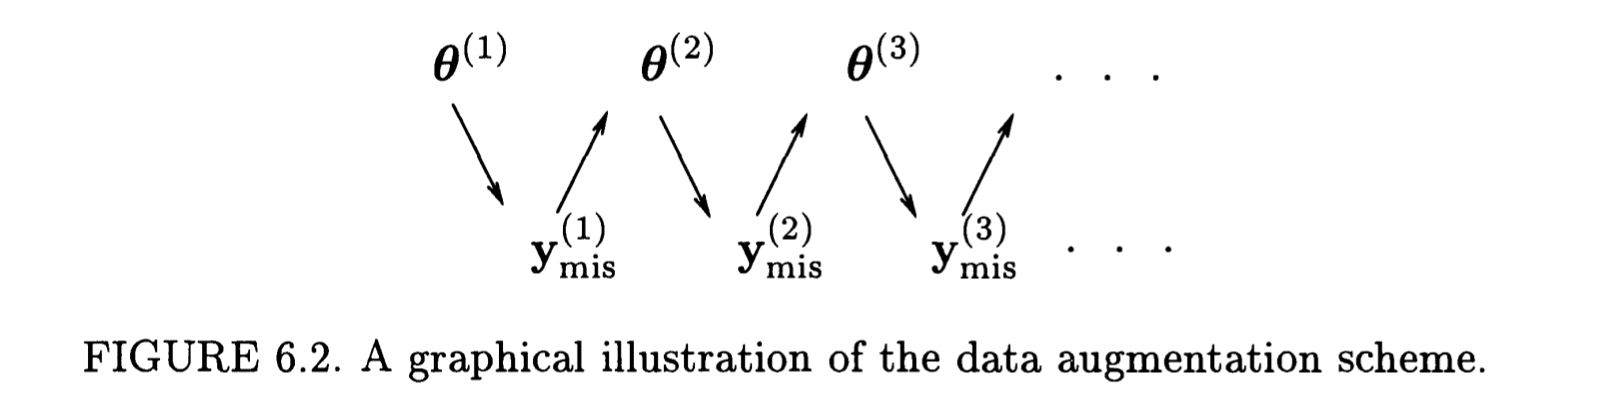
\includegraphics[scale = 0.5]{data_augmentation.png}}
\end{minipage}
\caption{\footnotesize{\textbf{Scheme for iteratively fill in missing data and update parameter \citep{liu2001monte}}}}
\label{fig: data_augmentation}
\end{figure}

\subsection{Monte Carlo EM}
\begin{itemize}
\item A difficulty with the implementation of the EM algorithm is that each "E-step" requires the computation of the expected log likelihood $Q(\mb{\theta}|\mb{\theta}_{0}, \mb{y})$. An alternative solution is to approximate the expectation via Monte Carlo simulation, i.e. 
\begin{align}
\widehat{Q}_{m}(\mb{\theta}|\mb{\theta}_{0}, \mb{y}) &= \frac{1}{m}\sum_{t=1}^{m}\ell_{c}(\mb{\theta}|\mb{X}_i, \mb{y}_i)
\end{align} where samples of missing data $\mb{X}_i \sim q(\mb{x}|\mb{y}_{i},\mb{\theta}_0), i=1,\ldots, m$.

\item As $m\rightarrow \infty$, $\widehat{Q}_{m}(\mb{\theta}|\mb{\theta}_{0}, \mb{y}) \rightarrow Q(\mb{\theta}|\mb{\theta}_{0}, \mb{y})$.


\end{itemize}


\newpage
\bibliographystyle{plainnat}
\bibliography{book_reference.bib}
\end{document}